\documentclass[12pt]{article}
\usepackage[a4paper]{geometry}
\usepackage[myheadings]{fullpage}
\usepackage{amsmath,amssymb,amsthm, enumitem, hyperref, tabto} 
\usepackage{fancyhdr}
\usepackage{arxiv}
\usepackage{lastpage}
\usepackage{graphicx, wrapfig, subcaption, setspace}
\usepackage[font=small, labelfont=bf]{caption} \usepackage{blindtext}
 \usepackage{blindtext}
\usepackage{url, lipsum}
\usepackage{tgbonum}
\usepackage{amsmath,physics}
\usepackage{authblk}
\usepackage{hyperref}
 \hypersetup{ 
     colorlinks=true, 
     linkcolor=blue, 
     filecolor=blue, 
     citecolor =red,       
     urlcolor=cyan,
     pdftitle={Using Spatial Trees to optimize Food Costs for Lower Wage Families}
     } 
\usepackage[super,compress,sort,numbers]{natbib}
\usepackage{csquotes}
\usepackage{multicol}
%\setlength{\multicolsep}{6.0pt plus 2.0pt minus 1.5pt}% 50% of original values
\usepackage{xcolor}
\usepackage{algpseudocode}
\usepackage{algorithm}
\floatname{algorithm}{Algorithm}
\usepackage{times}
\usepackage{adjustbox}
\usepackage[T1]{fontenc}
\usepackage{makecell}
\usepackage{parskip}
\usepackage{erewhon}
\usepackage{geometry}
\usepackage{caption}
\usepackage{subcaption}
\usepackage{framed}
\setlength\FrameSep{0.5em}
\setlength\OuterFrameSep{\partopsep}
% \usepackage{draftwatermark}
\graphicspath{ {./images/} }
\usepackage{sectsty}

\sectionfont{\fontsize{15}{20}\selectfont}
\usepackage{tikz}
\def\checkmark{\tikz\fill[scale=0.4](0,.35) -- (.25,0) -- (1,.7) -- (.25,.15) -- cycle;} 
\usepackage[sorting=none]{biblatex}
\addbibresource{references.bib}

\newcommand{\HRule}[1]{\rule{\linewidth}{#1}}
\onehalfspacing
\setcounter{tocdepth}{5}
\setcounter{secnumdepth}{5}

\renewcommand{\headrulewidth}{0pt}
\renewcommand{\footrulewidth}{0pt}

\begin{document}


\pagestyle{fancy}
\fancyhf{}
\fancyhead[L]{\footnotesize \textbf{CS5132} PA2 - \emph{Using Spatial Trees to optimize Food Costs for Lower Wage Families} }

\fancyfoot[R]{Page \thepage\ of \pageref{LastPage}}


{\selectfont
\title{
	\huge \textbf{Using Spatial Trees to optimize Food Costs for Lower Wage Families}
}

\date{}

\author[1]{Kannan Vishal}
\author[1]{Prannaya Gupta}
\author[1]{Quek Yu Pin}
\author[1]{Vikram Ramanathan}
\affil[1]{NUS High School of Math and Science}

\maketitle

\vspace{-2cm}

\tableofcontents

\thispagestyle{empty}
\newpage

\section{Background}

Lower income families are plagued by food expenses nowadays, with it making up a significant proportion of their monthly expenditures. Frequently, one's choice of grocery-outlet is largely determined by convenience, e.g. going to the nearest \textit{7-Eleven}. On the other hand, walking a bit further to the closest \textit{FairPrice} is also a valid option, as compared to other nearby sources that tend to mark up their products. But what if such families enter a neighbourhood they are unfamiliar with? How can they be sure that they can get meals for affordable prices? In this report, we design a platform to present and compare such options in a relatively concise interfaces, that allows selection based on \textbf{both price and distance}. This selection is done via the use of Spatial R-Trees and QuadTrees. Of course, this is not limited to food; this platform can be extended to work with any type of commodity. In this way, users can make more informed decisions regarding their expenditures.
    
   
\section{User Documentation}
You are to provide a brief user documentation with \textbf{screenshots} on how to use the
program and its functionalities.

\section{Analysis and Explanation of Implemented Tree Methods}

Provide a brief explanation, in your own words, and rigorous mathematical worst-case
analysis derivation and time complexity of the key methods of your tree structure
(retrieval, insertion, deletion, balance (if any))



\subsection{Spatial Quad-Trees}
\begin{figure}
    \centering
    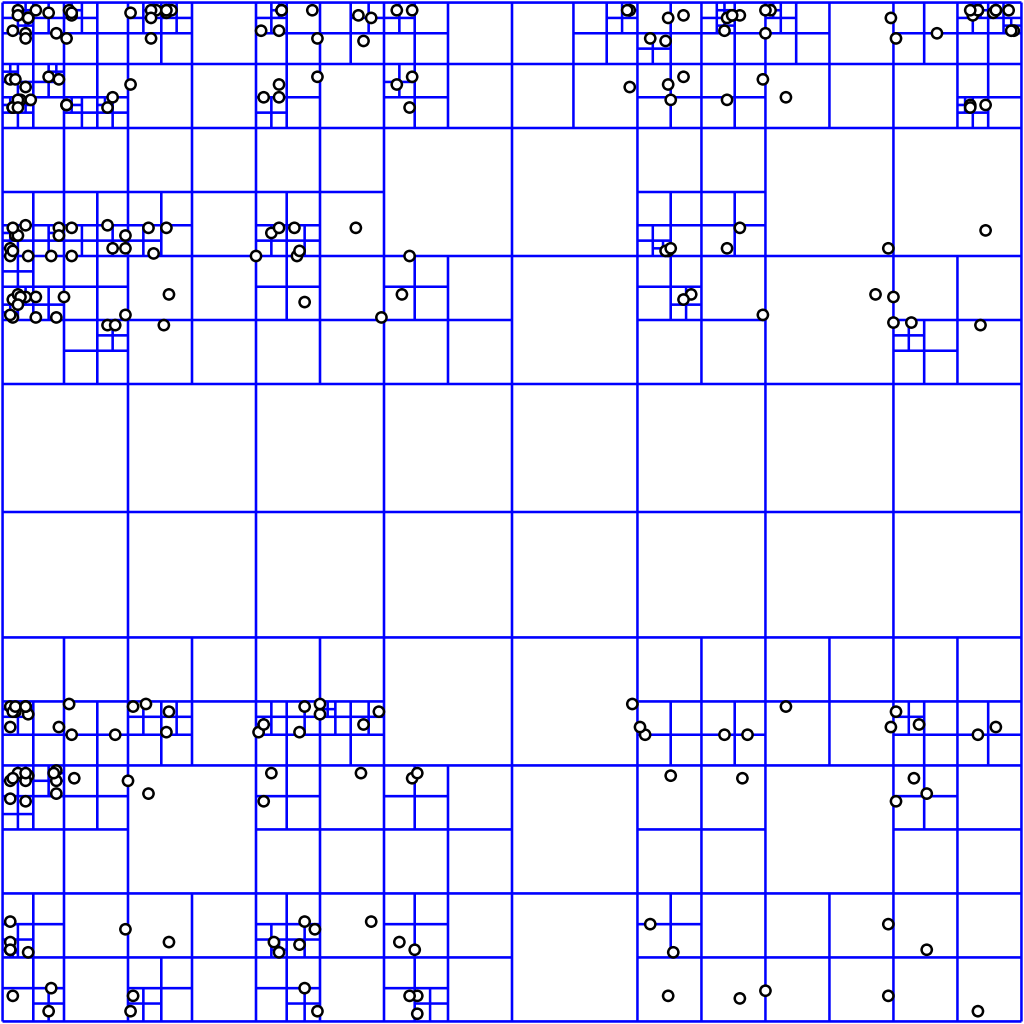
\includegraphics[scale=0.3]{../img/quadtree.png}
    \caption{Quad-Tree visualization}
    \label{fig:my_label}
\end{figure}
Quad-Trees are commonly used in analysing the distribution of a collection in 2D space, as the size and precision of the data structure scales with the distribution of the spatial data we are working with. As we map out store branches over Singapore, we may find that the locations are not evenly distributed. If we try to split up the map of Singapore into a grid, and check if each grid is occupied by a store, then we may have a lot of overlap of stores in shopping districts, and wasted space in more residential areas.

\subsubsection{Why Quad-Trees?}

So, given the above issues, why did we choose Quad-Trees? Quad-Trees address this by adopting a recursive subdivision approach to grid-propagation. That is, a quadrant is subdivided only during when there is a child node to be inserted into the quadrant. The depth of the tree is thus proportional to the log of the local density of points, which results in many speedups. Empty areas have very low depth, and dense areas have fewer "collisions".

This is particularly relevant in our case, because stores selling goods are very much not uniformly distributed throughout space. Many parts of Singapore, such as housing areas, will obviously have a relatively lower density of food-sellers than a large shopping mall. There is a hierarchy to be found here, too. While Quads obviously do not perfectly represent buildings, a resolution of 50 meters ensures that a building is likely to take up a subtree of depth 1-2 at the most. The implicit ordering follows upwards: A few of these subtrees form a series of blocks, these blocks form an area, and so on and so forth. While this is more a reflection of the choice of 50 meters than anything else, the arrangement is still noteworthy. It also, being a relatively small number, ensures that a Quad will not have too many stores in it.

\subsubsection{Algorithm}

In terms of implementation, Quad-Trees are a generalisation of binary search trees to two dimensions. In order to facilitate this, internal nodes in the Quad-Trees have four children rather than two. Naturally however, one has to ask: how are we ordering objects in two dimensions? It is common knowledge that extending from the reals to the complex numbers gives up natural ordering, and the same applies here. Well, I'm so glad you asked, dear reader. Think about it: what do we actually use ordering for in a binary search tree? We use it to figure out if an element goes left or right. And here? Well, if we're using ordering to partition, why not just partition without ordering? And so we do, recursively subdividing quads into 4 smaller quads when necessary.

Insertion begins with a little preamble. If the object (the object in question is termed a SuperStore) to be inserted has a position that is outside of the bounding box of the Quad-Tree's root node, an exception is immediately thrown. Otherwise, the appropriate QuadNode child of the current node is chosen, created if it is currently null, and recursed on if it has an item (even if that item is null). When we reach a node that already has an item in it, we simply subdivide that node, and then reallocate both the current item and the previously stored item. Essentially, what this does is ensure that the depth of the tree is both \textbf{Dynamic} and \textbf{Local}. Naturally, you may wonder, "What if two SuperStores have the same position"? Well, for that, we have a minimum Quad size. This minimum Quad size is about 0.00045 degrees (latitude and longitude), which translates to a resolution of roughly 50 meters.

Naturally, however, this raise another problem: How do we store multiple SuperStores in a single QuadNode? After all, as per the specifications of this assignment, QuadNode must extend Node, and Node only holds a single object of type T. Must we store an ArrayList of SuperStores? The answer is, kind of. You see, each SuperStore holds an Arraylist of items. And now you see why it's called a SuperStore; when two SuperStores would take up the same minimum-sized node, they instead merge their catalogues together. For this to work nicely, items must store their location so that what store they actually belong to can be ascertained, and indeed they do. While this is not the most space-efficient approach, the space required to store this information is not huge in the grand scheme of things.

That more or less covers insertion. As there is no deletion operation (it doesn't make sense in this context), that leaves only window queries.

The process for doing window queries is rather intuitive. We start at the root, where we iterate over all children. If a given child quad has overlap with the query area, we recurse on it, passing down a shared Arraylist of items. If not, we skip the child. Whenever we reach a child that has an object inside of it, we append all of its items (that are inside of the query area) to the Arraylist. Repeat, until all quads overlapping the query have been traversed. This Arraylist is finally returned when the recursion terminates.

\subsubsection{Time Complexity}

\paragraph{Insertion:} 

The worst-case time complexity of the insertion operation for Quad-Trees is O(n).

First, let us observe that no matter the structure of the tree, at most a finite number of recursive calls will be made to propagate down it. Due to the minimum size of the lowermost QuadNode, once we reach a depth of around 10 (because Singapore is roughly 50km across), we will hit the minimum size. However, since this is a finite distance, this only contributes a constant term to the asymptotic time complexity of the algorithm. Indeed, 10 is low enough that we can call it constant without feeling bad about it. More relevant here is the merge operation.

Because we merge the the two catalogues together, we invariably invoke java's System.arrayCopy method. In researching the time complexity of this method, I have come to the conclusion that the only explanation here is "It's complicated". Given this, we will make the safe assumption that it is still O(n), where n is the number of elements to be moved from one array to another. \newline
The time taken to run System.arrayCopy is then roughly of the form:
$$T(n) = an + 10b + c$$
Where a is the constant factor hidden behind O(n), b is the time taken to run one recursive call, and c is whatever other overhead we have. If we accept this, then the asymptotic worst-case time complexity of insertion is:
$$O(n)$$
// Insert rigorous analysis of range queries here

%\subsection{Spatial R-Trees}

%\begin{figure}
    %\centering
    %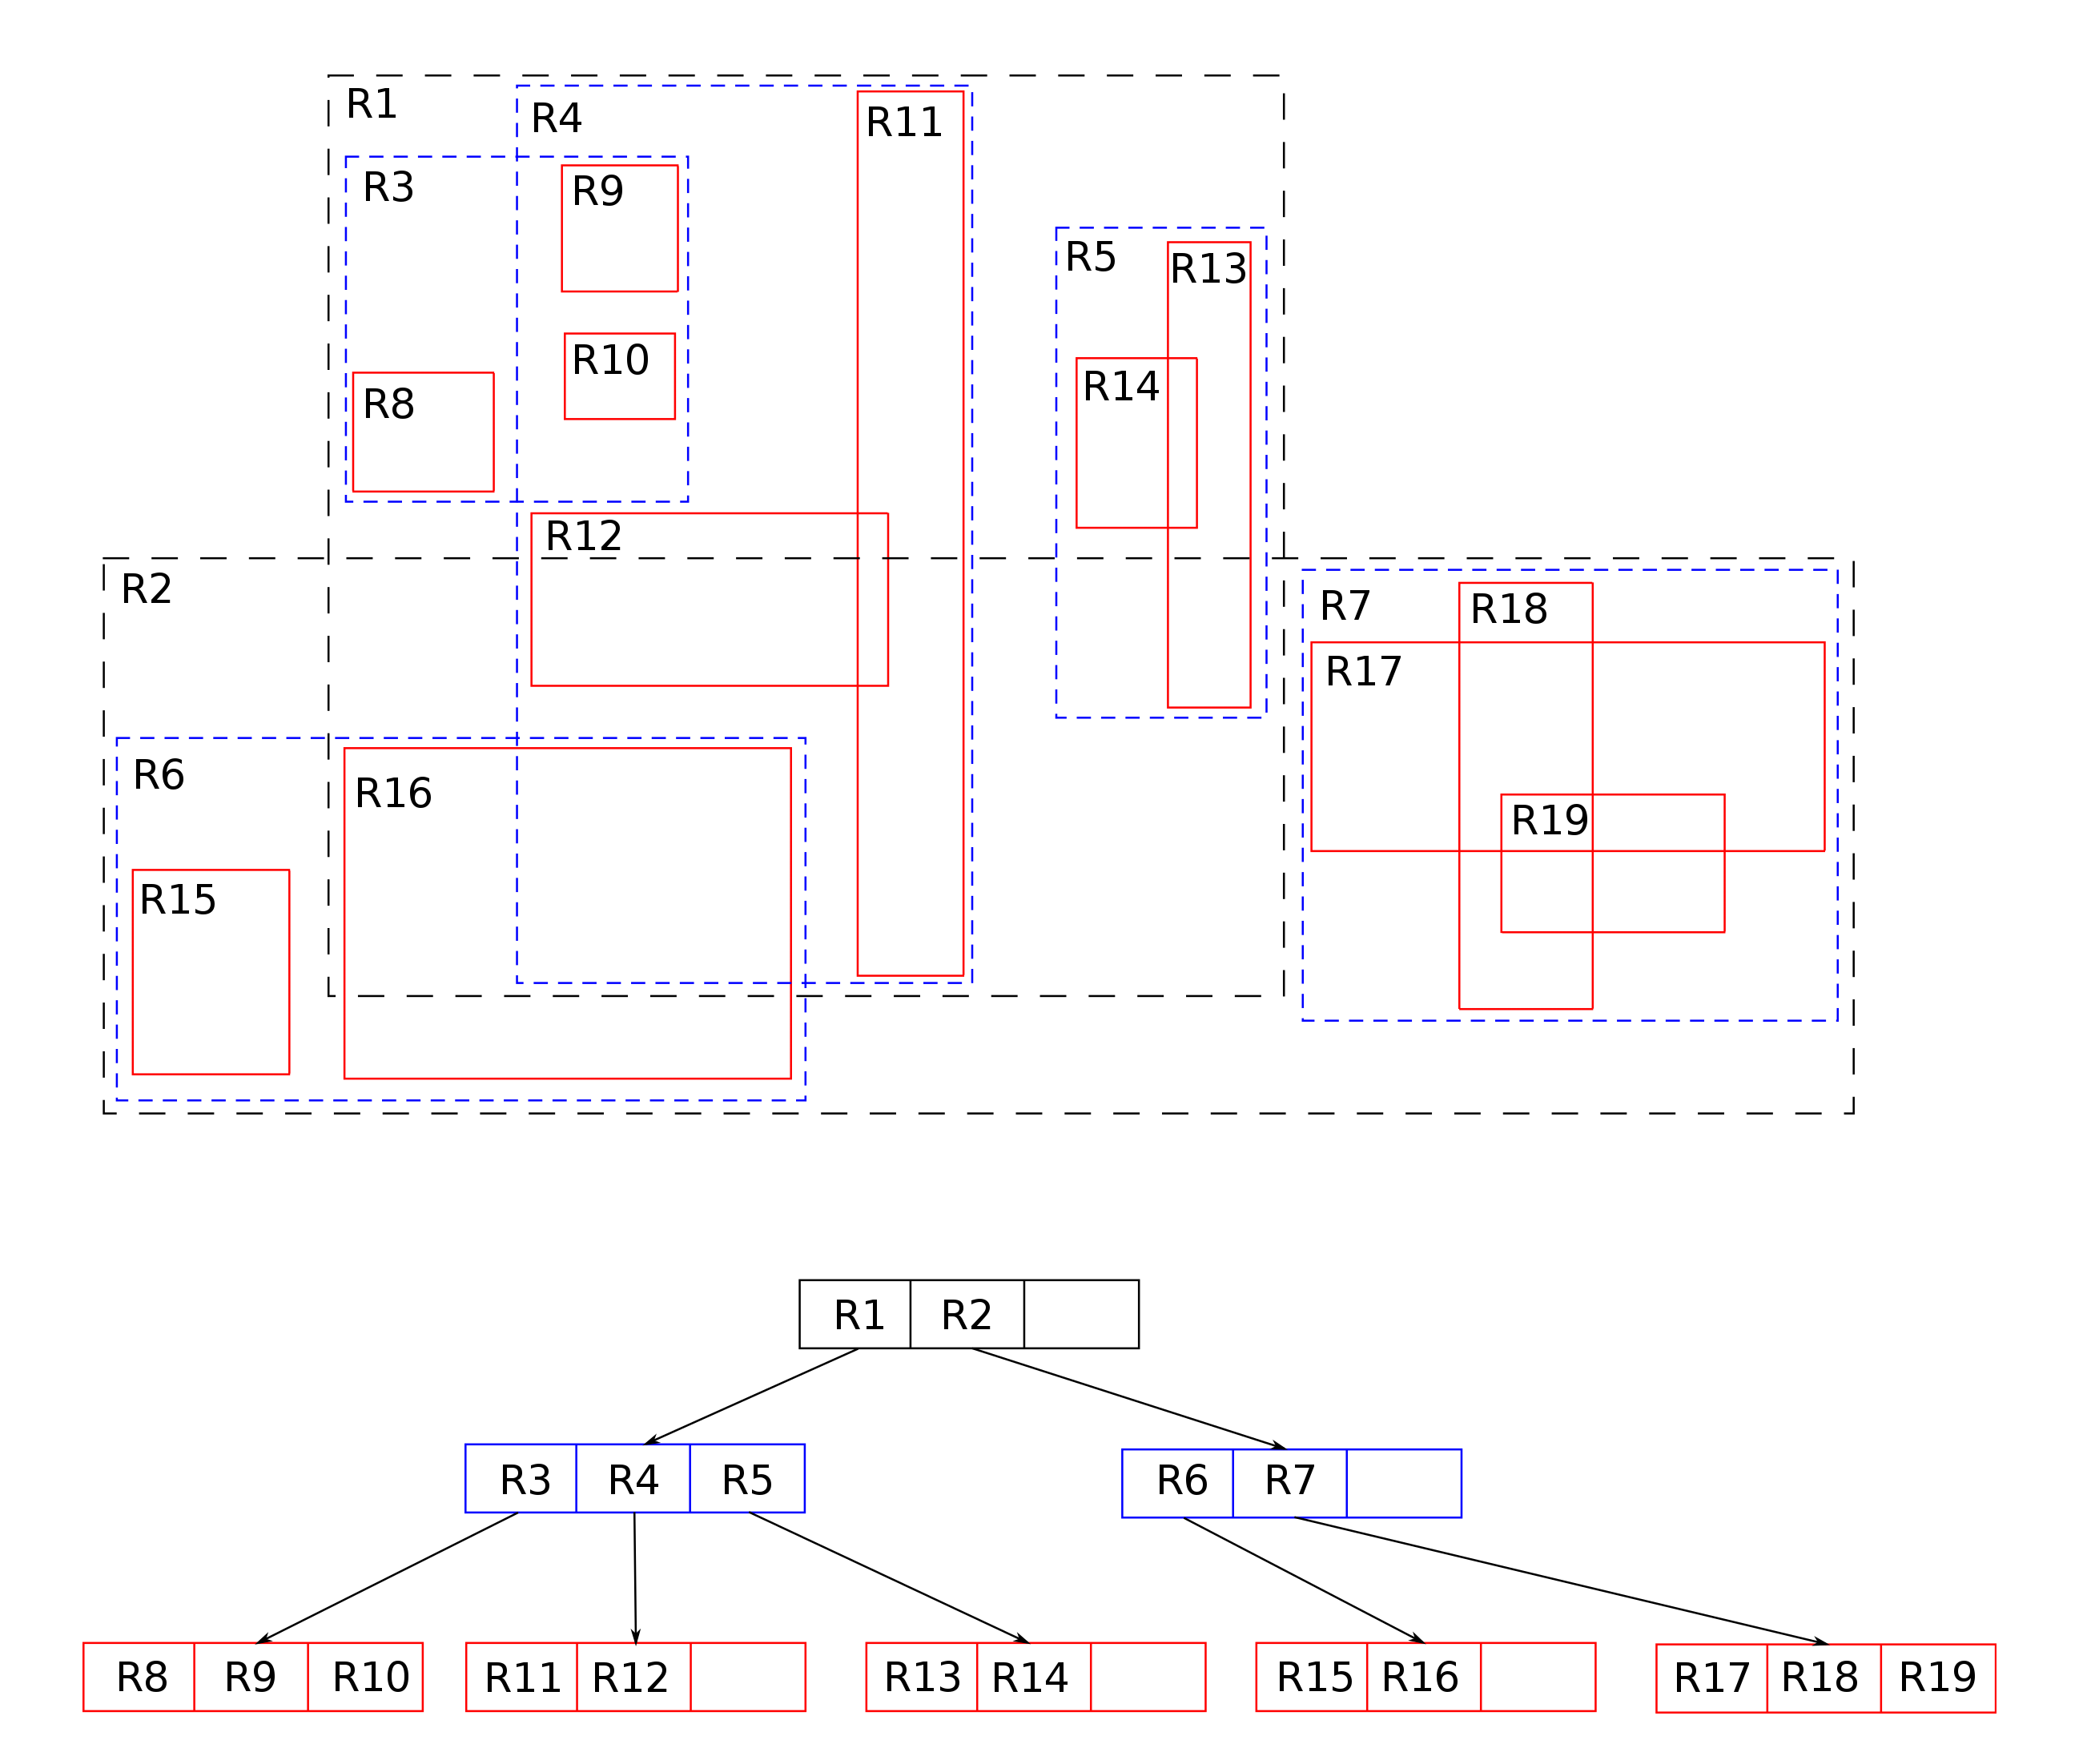
\includegraphics[scale=0.3]{../img/RTree.png}
    %\caption{R-Tree visualization}
    %\label{fig:my_label}
%\end{figure}

%Another approach to storing points in space, especially for our purposes of nearest neighbour queries, is to group points together, according to their closeness, and then recursively group those groups together. 

%\subsubsection{Algorithm}



%\subsection{R-Trees vs. Quad-Trees}


% Hypothesis
% Why we think one would work better


\section{Testing Strategy}
You are to provide at least \textbf{3 test cases} you used to test the correctness and
robustness of your program. Log down the sample input and output for each test case.
Briefly explain why each test case was chosen.



\section{Results}

% Which data structure did better

\newpage
\section{GitHub Information}
You can find our repository at \url{https://github.com/ThePyProgrammer/SnackNow}.

\subsection{User Directory}
\begin{center}
    \begin{tabular}{|c|c|}
        \hline
        GitHub Username & Real Name \\
        \hline
        \href{https://github.com/delargement}{\texttt{delargement}} & Kannan Vishal \\
        \href{https://github.com/ThePyProgrammer}{\texttt{ThePyProgrammer}} & Prannaya Gupta \\
        \href{https://github.com/h1810126}{\texttt{h1810126}} & Quek Yu Pin \\
        \href{https://github.com/VikramRamanathan}{\texttt{VikramRamanathan}} & Vikram Ramanathan \\
        \hline
    \end{tabular}
\end{center}


\subsection{Repo Report}

\section{Reflection}

\subsection{Vishal}

By helping out a here and there in each component of the project, and reviewing our project while writing the report, I have gained a better understanding of the software development lifecycle, from the brainstorming stage, UI prototyping stage, data collection and documentation. By abstracting each component of the project, such as the model (RTree and Quadtree implementation) and GUI, and distributing the workload, we were able to be more productive, and it was enjoyable to see each of the pieces to connect together to give a minimum viable product.

\subsection{Prannaya}

\subsection{Yu Pin}

\subsection{Vikram}

\section{Work Distribution Matrix}

\begin{center}
\begin{tabular}{|c|c|c|c|c|}
    \hline
    & Vishal & Prannaya & Yu Pin & Vikram \\ [0.5ex] 
    \hline\hline
    Ideation & &  &  & \checkmark \\
    R-Tree Implementation &  & \checkmark &  &  \\
    Quad-Tree Implementation &  &  &  & \checkmark \\
    Data Collection &  &  & \checkmark &  \\
    User Interface  & \checkmark & \checkmark &  &  \\
    Report  & \checkmark & \checkmark  &  & \checkmark  \\
    \hline
\end{tabular}
\end{center}


\newpage


\section{References}

\printbibliography[
heading=none
]
}

\end{document}